\cotefile{34}
\scanpage{116}
\mspage{31}
% archive sheet number: 115

% L01-04
\uline{Corollaire} 4.\unsure{7}. \unsure{Dans|Sous} les conditions de 4.4, supposons $X\inserted{=\operatorname{Spec} A}$ \unsure{strictement} local et satisfaisant au\deleted{x conditions du} th. de pureté cohomologique. Soit $m$ un \deleted{\unsure{entier, qui}} multiple de $n$, premier à la car. résiduelle de $X$, et soit

% L05
\[
\unsure{X'_m|X'}=\operatorname{Spec} A[T_1,\ldots,T_r]/(T_1^m-\unsure{a_1|g_1},\ldots,T_r^m-a_r),
\]

% L06-07
où \deleted{\unsure{pour}} les $a_i$ sont des équations \deleted{\unsure{les}} des $D_i$ $(1\leq i\leq r)$. Soit $U'=X'\times_X U$, Alors l'homomorphisme \unsure{canonique}

% L08
\[
H^*(U,\Lambda)\unsure{{-}|\longrightarrow}H^*(U',\Lambda)
\]

% L09
est nul en dimensions $>0$.

% L10-12
En effet, c'est trivial en dim. 1, car (4.5.1) \deleted{\unsure{dit}}\inserted{équivaut} précisément \inserted{à dire} \deleted{\unsure{que nous}} que $U'$ est un revêtement \deleted{\unsure{galois}} principal connexe, de groupe $\unsure{\mu_n|\mu_m}$.

% L13-14
\deleted{4.8. Soit maintenant $X$ \unsure{str.} local régulier satisfaisant au th. de pureté cohomologique.}

% L15-18
4.8. Soit $X\inserted{=\operatorname{Spec} A}$ un schéma strictement local régulier, $(a_i)_{1\leq i\leq r}$ une partie d'un système régulier de paramètres de $A$, de sorte que \deleted{\unsure{les}} \deleted{$D=\operatorname{div}(a_i)$}

% L18
\[
\boxed{D=\operatorname{div}\left(\prod a_i\right)=\sum D_i\qquad (\text{où }D_i=\operatorname{div}a_i)}\quad\deleted{\unsure{est}}
\]

% L19-20
est un diviseur à croisements normaux, à composantes premières $D_i$ régulières. Posons encore

% L21
\[
\boxed{U=X-\operatorname{supp}D=X-\bigcup D_i},
\]

% L22-24
\deleted{\illegible{1}} et pour tout entier $m$ premier à la car. résiduelle de $X$, introduisons
\[
X(m)=\operatorname{Spec}A[T_1,\ldots,T_r]/(T_1^m-a_1,\ldots,T_r^m-a_r),
\]

\scanpage{117}
\mspage{32}
% archive sheet number: 116

% L01-05
et l'image inverse $U(m)$ de $U$ dans $X(m)$, qui est un rev. étale \deleted{\unsure{pr.}} principal de $U$ de groupe $\mu_m(X)^r=G(m)$, les $U(m)$ forment un syst. projectif de \deleted{\unsure{schémas affines}} \unsure{revêts} étales \deleted{\unsure{et}} principaux, compatibles avec les hom de transition évidents

% L06-07
\diagram{\begin{tikzcd}[ampersand replacement=\&]
\mu_{m'}^r(X)\arrow[r,no head]\arrow[d,equal]\&\mu_m^r(X)\arrow[d,equal]\\
G(m')\&G(m)
\end{tikzcd}}
\inserted{pour} $(m\mid m')$.

% L08-09
Soit \deleted{$\unsure{U(\infty)}$}
\[
U(\infty)=\varprojlim U(m)
\]

% L10-11
qui est un \deleted{\unsure{revêtement proétale de}} pro-revêtement étale de $U$ de groupe

% L12
\[
G\deleted{(\unsure{\infty})}=\varprojlim_m G(m)=\prod_{\ell\ne p}\unsure{\mathbb{Z}|Z}_\ell(1)^r,
\tag*{(4.8.1)}
\]

% L13-14
\inserted{$p$ est la car. résiduelle de $X$, et où} où l'on pose par définition

% L15
\[
\mathbb{Z}_\ell(1)=\varprojlim_\nu\mu_{\ell^\nu}(X).
\tag*{(4.8.2)}
\]

% L16-17
Soit $n$ un entier $>0$ fixé tel que $n$ soit premier à $p$, \inserted{et soit encore $\Lambda=\mathbb{Z}/n\mathbb{Z}$.} On a donc

% L18
\[
H^*(U(\infty),\Lambda)\simeq\varinjlim_m H^*(U(m),\Lambda),
\tag*{\unsure{(*)|(1)}}
\]

% L19-23
\deleted{et \unsure{compte tenu} que}
\[
\deleted{U(m)=X(m)-\bigcup_{1\leq i\leq r}D'_i(m),}
\]
\deleted{avec $X(m)$ régulier et les $D'_i(m)\inserted{=\operatorname{div}(T_i(m))}$ des diviseurs réguliers dont la somme est à croisements normaux, on trouve que}

% L23-24
D'autre part, d'après les rappels de 4.6, le calcul de l'hom de transition

\scanpage{118}
\mspage{33}
% archive sheet number: 117

% L01
\[
H^*(U(m),\Lambda)\unsure{{-}|\longrightarrow}H^*(U(m'),\Lambda),\quad\text{pour }m\mid m'
\]

% L02-04
est justiciable de 4.6 (où on \deleted{\unsure{prendra}}\inserted{\unsure{remplacera|remplace}} $n$ par $m'/m$), donc est nul \inserted{en degrés $\ne0$}, si $nm\mid m'$, \inserted{sous réserve du th. de pureté \unsure{coh.|ch.}} \deleted{D'ailleurs,} Cela prouve que le deuxième \unsure{mbr} de $(*)$ est nul en dim $>0$, et en dim. 0 il est évidemment isomorphe à $\Lambda$. Donc on trouve

% L05-07
\uline{Corollaire} 4.9. Dans les notations de 4.8, et supposant que $X$ et les $X(m)$ satisfont au th. de pureté coh., \deleted{\unsure{on dit}} on a

% L08-09
\[
\left\{\begin{aligned}
H^i(U(\infty),\Lambda)&=0\quad\text{si }\deleted{\unsure{\Lambda}}\ i\ne0\\
H^0(U(\infty),\Lambda)&\simeq\Lambda
\end{aligned}\right.
\tag*{(4.9.1)}
\]

% L10-14
\deleted{\uline{Remarques} 4.10.\unsure{a)} Si on suppose seulement que les $X(m)$ satisfont au th. de pureté \inserted{coh.} en dim $\leq N$ (condition vide si $N=1$ !), alors on trouve que (4.9.1) est encore vrai si $i\leq N$.}

% L15-17
\deleted{b) On peut exprimer encore de façon imagée le résultat de 4.9 en disant que \inserted{\unsure{à $p$-torsion près}} \unsure{cohomologiquement} $U$ se comporte comme un}

% L18-19
\uline{Corollaire} 4.10. \inserted{Sous les conditions de 4.9,} Soit $\Gamma$ un groupe profini, considérons un homomorphisme de groupes profinis

% L20
\[
\unsure{\varphi|\phi}:G\deleted{(\unsure{\infty})}\longrightarrow\Gamma,
\tag*{(4.10.1)}
\]

% L21
et soit $H$ le noyau de cet homomorphisme.

\scanpage{119}
\mspage{34}
% archive sheet number: 118

% L01-03
\deleted{Alors} Considérons l'\inserted{anneau de} cohomologie $H^*(H,\Lambda)$, sur lequel \unsure{on} fait opérer $G\deleted{(\unsure{\infty})}$ trivialement, et considérons l'anneau induit

% L04
\[
H^*(H,\Lambda)\mathbin{\times^{G\deleted{(\infty)}}}\Gamma.
\]

% L05-06
\deleted{Alors} Considérons d'autre part le revêtement principal $\overset{\deleted{\unsure{\sim|\infty}}}{U}'$ de groupe $\Gamma$

% L07
\[
\overset{\deleted{\sim}}{U}'=U(\infty)\mathbin{\times^{G\deleted{(\infty)}}}\Gamma
\]

% L08
associé à $U(\infty)$ de groupe $G\deleted{(\infty)}$, et l'hom $G\deleted{(\infty)}\unsure{{-}|\longrightarrow}\Gamma$.

% L09-11
On a alors un homomorphisme canonique d'anneaux \inserted{\unsure{gradués à opérateurs} $\Gamma$}. \unsure{Faisons|Faisant} opérer $\Gamma$ sur l'anneau $H^*(\widetilde U,\Lambda)$ via \inserted{ses opérations sur $\widetilde U$}

% L12
\[
H^*(\unsure{U'|\widetilde U'},\Lambda)\simeq H^*(H,\Lambda)\mathbin{\times^{G\deleted{(\infty)}}}\Gamma.
\tag*{(4.10.1)}
\]

% L13
\deleted{En particulier, si $\deleted{\unsure{K}}\Gamma'$ est l'image $G\deleted{(\infty)}$ dans $\Gamma$, le \unsure{groupe} $\Gamma'$ est \unsure{H}}

% L14
\uline{Démonstration} \deleted{C'est une conséquence triviale}

% L15
Soit $K=G\deleted{(\infty)}/H=\operatorname{Im}(G\deleted{(\infty)}\to\Gamma)$. Alors

% L16
\[
U'=(\unsure{U^\infty|U'}/H)\mathbin{\times^K}\Gamma,
\]

% L17
et par suite on trouve un isom \inserted{d'anneaux gradués à groupe d'op. $\Gamma$}
\[
H^*(U',\Lambda)\simeq H^*(U^\infty/H,\Lambda)\mathbin{\times^K}\Gamma
\]

% L18-21
où $K$ opère sur $H^*(U/H,\Lambda)$ via ses opérations sur $U/H$. Si nous prouvons que ces dernières sont \deleted{\unsure{nulles}}\inserted{triviales}, \deleted{\unsure{on en conclura}} et qu'on a un isom d'anneaux gradués $H^*(U^\infty/H,\Lambda)\simeq H^*(H,\Lambda)$, on aura terminé.

% L22-24
Cela nous ramène au cas où (4.10.1) est \uline{surjectif}. Alors la suite spectrale déduite de Hochschild Serre (SGA 4 \uline{VII} $\ldots$) est

% L25
\[
H^*(U^\infty/H,\Lambda)\Longleftarrow E_2^{pq}=H^p(H,H^q(U(\infty),\Lambda)),
\]

\scanpage{120}
\mspage{35}
% archive sheet number: 119

% L01-03
jointe à 4.9, \inserted{qui implique que $E_2^{pq}=0$ si $q\ne0$,} donne l'isomorphisme voulu d'anneaux gradués :
\[
H^*(U^\infty/H,\Lambda)\simeq H^*(H,\Lambda).
\]

% L04-09
D'autre part, cet isom transforme, comme il est bien connu, les opérations de $G\deleted{(\unsure{\infty})}/H$ sur le premier mbr en les opérations déduites des opérations de $G\deleted{(\infty)}$ sur $H$ par autom. intérieurs. Comme $G\deleted{(\infty)}$ est commutatif, cette action est triviale, ce qui achève la démonstration de 4.10.

% L10-14
% relocation arrow from crossed Corollaire 4.12 toward the position before Remarque 4.12
\margin{\figure{\begin{tikzpicture}[scale=.45]\draw[->] (0,-2) to[out=150,in=220] (0,2);\end{tikzpicture}}}
\uline{Remarque} 4.12. Si on suppose seulement que les $X(m)$ satisfont au th. de pureté coh. en dim $\leq N$, alors les arguments qui précèdent prouvent encore 4.9 à 4.11 en dim $\leq N$, \deleted{et par suite aussi le corollaire 4.13 qui suit.}

% L15-18
\uline{Corollaire} 4.11. \deleted{4.12.} \inserted{Soit $\Gamma'$ l'image de $G\deleted{(\infty)}$ dans $\Gamma$, et} Supposons $\Gamma$ commutatif (ou plus gén. \deleted{l'image de $G(\infty)$ dans $\Gamma$}\inserted{$\Gamma'$ invariant dans $\Gamma$})\deleted{\unsure{invariant}}. Alors, l'action de $\Gamma$ sur $H^*(U',\Lambda)$ induit sur $\Gamma'$ l'action triviale (plus précisément $\Gamma'$ est le s-groupe des $g\in\Gamma$ qui opèrent trivialement sur $H^*(U',\Lambda)$).

% L19-24
Cet énoncé suffira \deleted{\unsure{pour le}} pour prouver \deleted{4.13. Nous \unsure{prouverons} maintenant} \deleted{plus bas} plus bas le th. de monodromie sous la forme 3.2. Avant de le faire, explicitons le calcul de $H^*(U',\Lambda)$ résultant de (4.10.1), ce qui nous sera utile dans l'exposé suivant.

\scanpage{121}
\mspage{36}
% archive sheet number: 120

% L01-02
4.13. Gardons les hypothèses de 4.9, \deleted{en supposant de plus $n$ de la forme $\ell^{\nu+1}$, et}

% L03
\[
\deleted{\Lambda=\unsure{\mathbb{Z}|Z}/\ell^{\nu+1}\mathbb{Z}}
\tag*{\deleted{(4.13.1)}}
\]

% L04-05
Le groupe commutatif $H$ se décompose en le produit de ses composantes $\ell$-primaires $H(\ell)$,

% L06
\[
H=\prod_{\ell\ne p}H(\ell),\qquad H(\ell)\subset G\deleted{(\unsure{\infty})}(\ell)\simeq\deleted{\unsure{\mathbb{Z}}}\mathbb{Z}_\ell(1)^r.
\]

% L07
Donc \uline{$H(\ell)$ est un module libre sur $\mathbb{Z}_\ell$ de rang} $\leq r$.

% L08-10
On en conclut \unsure{quasi} aussitôt, si \deleted{$\Lambda=\mathbb{Z}/n\mathbb{Z}$ avec $n=\unsure{\ell^{\nu+1}}$}, \deleted{$\Lambda$ est un $\unsure{\ell|\mathbb{Z}}$ groupe} \deleted{\unsure{fini annulé par une puissance de} $\ell$}
\[
\Lambda=\mathbb{Z}/n\mathbb{Z},\quad\text{avec }n=\ell^{\nu+1}
\tag*{(4.13.\unsure{2})}
\]

% L11-12
\[
\left\{\begin{aligned}
H^*(\deleted{\unsure{\Lambda}}H,\Lambda)&\simeq\bigwedge^*H^1(H,\Lambda)\deleted{\unsure{\otimes\Lambda}}\unsure{,|/}\\
H^1(H,\Lambda)&\simeq\operatorname{Hom}(H,\Lambda)\simeq\deleted{\unsure{\mathbb{Z}|*}}\Lambda^s,\quad\text{où }H(\ell)\simeq\mathbb{Z}_\ell^s.
\end{aligned}\right.
\tag*{(4.13.1)}
\]

% L13-15
4.14. \deleted{Soit maintenant} \deleted{\unsure{Si nous}} Supposons maintenant donnés des entiers $m_i\geq0$ $(1\leq i\leq r)$, et \deleted{considérons} soit
\[
\deleted{\unsure{y}}\quad t=a_1^{m_1}\cdots a_r^{m_r}
\tag*{(4.14.1)}
\]

% L16-17
Soit, pour tt entier $m$ premier à la car. résiduelle de $X$
\[
X'(m)=\operatorname{Spec}A[T]/(T^m-t)
\tag*{(4.14.2)}
\]

% L18-19
et \deleted{considérons}
\[
\deleted{Y=}\quad\deleted{U(m)}\quad U'(m)=X'(m)\times_X U,
\tag*{(4.14.3)}
\]

% L20-22
qui est un revêtement étale principal \inserted{de $U$,} de groupe $\mu_m(X)$. Pour $m$ variable, les \inserted{$X'(m)$ et les} $U'(m)$ forment un syst projectif, et on trouve à la limite un

% L23
\[
U'=\varprojlim_m U'(m),
\tag*{(4.14.4)}
\]

% L24-25
qui est un schéma principal sur $U$ de groupe
\[
\Gamma=\deleted{\unsure{\mathbb{Z}_p}}\varprojlim\mu_m(X)=\prod_{\ell\ne p}\mathbb{Z}_\ell(1).
\tag*{(4.14.5)}
\]

\scanpage{122}
\mspage{37}
% archive sheet number: 121

% L01-02
Ce revêtement est de la forme
\[
U'=U(\infty)\mathbin{\times^G}\Gamma,
\tag*{(}
\]

% L03-05
pour un hom $\unsure{\varphi|\phi}:G\to\Gamma$ dont le calcul est immédiat, et qui \deleted{\unsure{se}} s'explicite, moyennant (4.8.1) et (4.14.5), comme

% L06
\[
\varphi(\lambda_1,\ldots,\lambda_r)=\sum_1^r m_i\lambda_i.
\tag*{(4.14.6)}
\]

% L07-09
On en conclut alors de (4.10.1) et (4.13.1) le calcul de $H^*(U',\Lambda)$. On trouve en particulier, grâce à 4.11 :

% L10-16
\uline{Corollaire} 4.15. \inserted{Dans les notations de 4.14,} Soit $m$ le pgcd des $m_i$, \deleted{Alors} \deleted{\unsure{et}} $m'$ le morceau de $m$ premier à $p$, et $\Gamma'\inserted{=m'\Gamma=m\Gamma}$ le sous-groupe de $\Gamma\simeq\prod_{\ell\ne p}\unsure{\mathbb{Z}|Z}_\ell(1)$ d'indice $m'$. Alors le sous-groupe des éléments de $\Gamma$ qui opèrent trivialement sur $H^*(U',\Lambda)$ (où $\Lambda=\mathbb{Z}/n\mathbb{Z}$, $n>1$, $(n,p)=1$) est égal à $\Gamma'$. \deleted{Pour tout \unsure{ent. premier à}}

% L17
On notera que $\Gamma'$ est \uline{indépendant de} $\Lambda$, \unsure{i.e. de $n$}.

% L18-19
\deleted{4.16. Nous allons mettre \unsure{les résultats sous la forme d'un énoncé} \illegible{1}}

% L20-24
4.16. Nous allons mettre les résultats 4.14, 4.15 sous une forme \deleted{\illegible{1}} plus globale, qui nous sera utile. Pour ceci, supposons donné un schéma \inserted{régulier} $X$, \deleted{\unsure{un}} un diviseur $D$ sur $X$ à croisements normaux, et une section
\[
t\in\Gamma(X,\unsure{\mathcal{O}|\mathscr{O}}_X).
\]

% L25-26
\deleted{On suppose que $\unsure{\pi(t)|V(t)|(t)}$} \deleted{Soit $U=$}

\scanpage{123}
\mspage{38}
% archive sheet number: 122

% L01-02
Soit
\[
U=X-\operatorname{supp}D,
\]

% L03-04
et supposons que
\[
\deleted{\unsure{a}}t|U\in\Gamma(U,\unsure{\mathcal{O}|\mathscr{O}}_U^*),\quad\text{i.e. }\operatorname{supp}\operatorname{div}t\subset\operatorname{supp}D.
\]

% L05-08
\deleted{Posons, pour tout entier $m$ premier aux caractéristiques} Supposons pour simplifier \deleted{\unsure{qu'il existe} \unsure{$X$ est de car nulle}, \inserted{$X$, de car. nulle, \unsure{ou bien}} \unsure{qu'il existe au plus un nb premier} $p$ \unsure{qui ne soit inversible sur} $X$.} $V(t)$ soit de car. $p>0$ et que tt nb premier $\ell\ne p$ soit inversible sur $X$.

% L09-10
Pour tout \deleted{\unsure{nb premier}} entier $m>0$ premier aux car. résiduelles de $X$, \deleted{\unsure{posons}} soit

% L11-12
\[
\left\{\begin{aligned}
X'(m)&=\operatorname{Spec}\mathcal{O}_X[T]/(T^m-t)\\
U'(m)&=X'(m)\times_X U
\end{aligned}\right.,
\]

% L13-15
de sorte que les $U'(m)$ forment un système projectif de rev. \deleted{étales et} principaux de $U$, de groupes les $\mu_{m,U}$. On considère

% L16
\[
U'=\varprojlim U'(m),
\]

% L17-18
qui est principal sur $U$ de groupe \deleted{$\unsure{\mu_m}$} $G_U$, où
\[
G=\varprojlim\mu_m\deleted{\unsure{(X)}},
\]

% L19-20
et on \deleted{\unsure{suppose}} considère \unsure{le|la} \deleted{projection}\inserted{\unsure{composé|composée}}
\diagram{\begin{tikzcd}[ampersand replacement=\&]
U'\arrow[r]\arrow[rr,bend left=22,"f"]\&U\arrow[r]\&X.
\end{tikzcd}}

% L21-24
Soit $n\geq1$ premier aux car. résiduelles de $X$, et \deleted{$\Lambda=\unsure{\mathbb{Z}|Z}/n\mathbb{Z}$} $\Lambda=\mathbb{Z}/n\mathbb{Z}$, on s'intéresse aux faisceaux
\[
R^i f_*(\Lambda_{U'})|X_0,\qquad X_0=V(t)
\]

\scanpage{124}
\mspage{39}
% archive sheet number: 123

% L01
sur $X_0$, et à l'opération de $G|X_0$ sur ces faisceaux.

% L02-07
Pour toute composante irréductible $D_i$ de $D$, soit $m_i$ la multiplicité de \deleted{\unsure{ce}} $D_i$ dans $\operatorname{div}(\pi)$; Soit $m$ le ppcm des $m_i$, et soit $m'=m$ si $X$ de car. nulle, $m'=$ partie de $m$ première à $p=\operatorname{car}V(\pi)$ dans le cas contraire. Écrivons $G$ additivement et considérons le groupe proétale

% L08
\[
\deleted{\unsure{mG}}\qquad G'=m'G\inserted{=mG}\subset G
\]

% L09
sur $X$. \deleted{\unsure{qui}}

% L10-16
\uline{Corollaire} 4.17. Dans les \deleted{hypothèses}\inserted{hypothèses et notations} de 4.16, supposons de plus que pour tt localisé strict $\overline{X}^{\unsure{s|0|6}}$ de $X$ en un point de $X_0$, les $\overline{X}(m)$ définis en termes du diviseur induit $\overline{D}$ (cf. 4.8) satisfont au th. de pureté. Alors l'opération de $G'|X_0$ sur \deleted{\unsure{les}} $R^*f_*(\Lambda_{U'})|X_0$ est triviale.

% L17-18
Cela résulte aussitôt de 4.15 par localisation stricte.

% L19-21
% insertion attachment uncertain: phrase is between structure de and the R^*f_* line
\deleted{4.18. En fait, on peut préciser la structure de \inserted{comme faisceau d'anneaux gradués à groupe d'op. $G|X_0$} $R^*f_*(\Lambda_{U'})|X_0$, On trouve tout d'abord}

% L22
\[
\deleted{R^*f}
\tag*{\deleted{(4.18.1)}}
\]

\scanpage{125}
\mspage{40}
% archive sheet number: 124

% L01
5. \uline{Démonstration du théorème de monodromie.}

% L02-06
Nous pouvons maintenant prouver 3.2, en utilisant la suite spectrale (2.5\inserted{bis}) \inserted{de 2.10.} (pour $\nu$ variable). Les résultats du n° \deleted{\unsure{suivant}}\inserted{précédent} prouvent que les $(\underline{\Psi}_\nu^q)\inserted{_{\mathrm{tame}}}$ sont des faisceaux constructibles, donc les $E_2^{pq}$ \deleted{sont} (pour $\nu$ fixé) sont des groupes finis.

% L07-09
Donc, passant à la limite sur $\nu$, on trouve une suite spectrale, compatible avec les opérations de $I_t$ et \unsure{ce|même} de $\unsure{\pi|\Pi}$ tout entier

% L10
\[
\deleted{H^*(\overline U,\deleted{\unsure{\Lambda}}\unsure{\mathbb{Z}|Z}_\ell)^P\Longleftarrow\inserted{\unsure{E_2^{pq}=\varprojlim}}H^p(\overline X_0,(\underline{\Psi}^q)_{\mathrm{tame}})}
\tag*{\deleted{(5.1)}}
\]

% L11
\deleted{avec}
\[
\deleted{(\underline{\Psi}^q)_{\mathrm{tame}}=\varprojlim_\nu(\unsure{\overline{\underline{\Psi}}_\nu^q|\underline{\Psi}_\nu^q})_{\mathrm{tame}}}
\tag*{\deleted{(5.2)}}
\]

% L12
\[
H^*(\overline U,\mathbb{Z}_\ell)^P\Longleftarrow E_2^{pq}=\varprojlim_\nu H^p(\overline X_0,(\underline{\Psi}_\nu^q)_{\mathrm{tame}}).
\tag*{(5.1)}
\]

% L13-15
On a vu dans 4.17 que le s-groupe $I'_t\subset I_t$ opère trivialement sur les $\underline{\Psi}_\nu^q$ donc \deleted{\unsure{les}} sur les $E_2^{pq}(\nu)=H^p(\overline X_0,\underline{\Psi}_\nu^q)$, donc sur leur limite $E_2^{pq}$.

% L16-21
Donc $I'$ opère trivialement sur tous les termes de la suite spectrale (5.1), donc sur l'\deleted{\unsure{aboutissement}} gradué associé à l'aboutissement. Comme le \deleted{\unsure{filtré}} gradué est donné, \unsure{sauf extensions} à partir des facteurs, on a gagné.

\scanpage{126}
\mspage{41}
% archive sheet number: 125

% L01
6. \uline{Application aux faisceaux de cycles évanescents.}

% L02-05
6.1. Soit à nouveau $X$ de type fini sur $S$, \inserted{étant} strictement local, et soit $U$ un ouvert de $X_\eta$, que nous supposons \uline{régulier}. \inserted{Soit $Y=X-U$, et} Supposons qu'il existe un morphisme propre $p:X'\to X$, \deleted{tel que} avec $X'$ régulier, $p^{-1}(Y)$ un diviseur à croisements normaux,

% L05-08 left margin
\diagram{\begin{tikzcd}[ampersand replacement=\&]
X'\arrow[d,no head,"p"']\&U\arrow[l,hook]\arrow[d,no head,"\sim"]\\
X\arrow[d,"f"']\&U\arrow[l,hook]\\
S\&
\end{tikzcd}}

% L06-14
et $U'=p^{-1}(U)\unsure{{-}|\longrightarrow}U$ un isomorphisme. (On sait par Hironaka [\ ] qu'il en est ainsi si $S$ est excellent de car. nulle, et \deleted{sans doute} il semble plausible qu'il en est de même dès que $S$ est excellent, sans restriction de caractéristique. D'ailleurs l'hypothèse ``$S$ excellent'' est anodine, car on s'y ramène pour ttes ces questions qui nous intéressent par passage au complété). \deleted{Sous ces conditions} Choisissons un entier $\ell\ne p$, et considérons, pour \deleted{tout}\inserted{un} entier $q$ \inserted{fixé} les faisceaux

% L15
\[
\boxed{(\underline{\Psi}_\nu^q)_{\mathrm{tame}}=(\underline{\Psi}_\nu^q)^P}
\tag*{6.1.1}
\]

% L16-18
(invariants \inserted{dans $\underline{\Psi}_\nu^q$ sous l'action du} \unsure{par le} p-s-groupe de Sylow $P$ de $I$)\deleted{\unsure{dans}}, \deleted{\unsure{Pour}} relatifs aux coefficients
\[
\Lambda_\nu=\unsure{\mathbb{Z}|Z}/\ell^{\nu+1}\mathbb{Z}\qquad(\nu\geq0).
\]
\inserted{(cf. 2.6 bis)} Ils forment un système projectif de faisceaux de torsion sur $X_0$.

% L19
\uline{Théorème} 6.2 : Avec les notations précédentes :

% L20-23
(i) Les faisceaux $(\underline{\Psi}_\nu^q)_{\mathrm{tame}}$ sont constructibles, et \deleted{il} le système projectif qu'ils forment \deleted{\unsure{$\ell$-adique}} \deleted{\unsure{satisfait} la condition MLAR (SGA 5 V 2.1.1)}, \inserted{est AR-$\ell$-adique (SGA 5 V \unsure{3.7.c|3.2.c})}, donc définissent un faisceau $\ell$-adique constructible (SGA 5 VI 1.1)

% L24
\[
(\underline{\Psi}^q)_{\mathrm{tame}}=\varprojlim_\nu(\underline{\Psi}_\nu^q)_{\mathrm{tame}},
\]

\scanpage{127}
\mspage{42}
% archive sheet number: 126
\margin{\deleted{$(\unsure{m=q(q+1)|m-q(q+1)})$}}

% L01-04
(ii) Il existe un sous-groupe \inserted{ouvert} $I'$ de $I$, \deleted{et un entier \unsure{$m$}} tel que pour tout $\nu$, l'action de $I'$ sur $(\underline{\Psi}_\nu^q)_{\mathrm{tame}}$ soit unipotente d'échelon \deleted{$\unsure{q(q+1)/2}$} $q+1$. \deleted{Alors}\inserted{Alors} L'action de $I'$ sur $(\underline{\Psi}^q)_{\mathrm{tame}}$ est également unipotente d'échelon \deleted{$\unsure{q(q+1)/2}$} $q+1$.

% L05-06
\uline{Démonstration} Soient $g,g'$ les morphismes canoniques de $U_{\overline\eta_t}$ dans $X',X$. On a

% L06 left margin
\diagram{\begin{tikzcd}[ampersand replacement=\&]
X'\arrow[d,"p"']\&\\
X\&U_{\overline\eta_t}\deleted{\unsure{(K_t)}}\arrow[l,"g"']\arrow[ul,"g'"']
\end{tikzcd}}

% L07
\[
(\underline{\Psi}_\nu^q)_{\mathrm{tame}}=R^q g_*^{\deleted{\unsure{\prime|2}}}(\Lambda_\nu)|X_0
\tag*{(6.2.1)}
\]

% L08-09
et \deleted{par suite} d'autre part la suite spectrale de Leray du morphisme composé $g=pg'$ donne

% L10
\[
R^*g_*(\Lambda_\nu)=(\underline{\Psi}_\nu^*)_{\mathrm{tame}}\Longleftarrow\deleted{\unsure{E_2^{pq}}}\inserted{E_2^{pq}(\nu)}=R^p p_*(R^q g'_*(\Lambda_\nu^{\deleted{\unsure{q}}})).
\tag*{(6.2.2)}
\]

% L11-13
En vertu des \deleted{\unsure{résultats}}\inserted{calculs du § 4}, on trouve un s-groupe ouvert $I'$ de $I$ qui, \inserted{pour tt $q,\nu$,} opère \deleted{de façon unipotente d'échelon \unsure{$q+1$} sur}\inserted{trivialement sur} $R^q g'_*(\underline{\Psi}_\nu^q)$. Il s'ensuit que $I'$ opère \deleted{\unsure{de}}\inserted{trivialement} \deleted{de façon unipotente d'échelon $\unsure{(0+1)+(1+1)+\cdots+(q+1)}$} sur $E_2^{pq}(\nu)$, donc \deleted{sur} il opère de façon unipotente \inserted{d'échelon $q+1$} \deleted{\unsure{dans}}

% L14-15
\deleted{\unsure{échelon} $(\underline{\Psi}_\nu^q)_{\mathrm{tame}}$, avec pour échelon \unsure{$q+1$}}
\[
\deleted{(0+1)+(1+1)+\cdots+(q+1)=\frac{q(q+1)}{2}},
\]

% L16
ce qui prouve la première assertion de ii).

% L17-20
D'autre part, les calculs explicites du § 4 montrent que les $R^q g'_*(\unsure{\Lambda|\underline{\Psi}}_\nu^{\deleted{q}})|X'_0$ sont des faisceaux \uline{constructibles}, qui pour $\nu$ variable forment un faisceau \deleted{\unsure{const.}} $\ell$-adique (i.e. $R^q g'_*(\Lambda_{\nu'})|X'_0=(R^q g'_*(\Lambda_\nu)|X'_0)\otimes_{\Lambda_\nu}\unsure{\Lambda_{\nu\nu'}|\Lambda_{\nu'}}$ si $\nu\geq\nu'$).

% L21
En vertu de SGA 5 \uline{VI} 2.2, il s'ensuit que

\scanpage{128}
\mspage{43}
% archive sheet number: 127

% L01-04
les $R^p p_*(R^qg'_*(\Lambda_\nu))|X_0\inserted{=R^p p_*(R^qg'_*(\Lambda_\nu)|X'_0),\quad\text{(th. de chgt de base propre)}}$, pour $\nu$ variable, forment un système AR-$\ell$-adique de faisceaux sur $X$, donc il en est de même des $R^i g_*(\Lambda_\nu)|X_0=(\underline{\Psi}_\nu^i)_{\mathrm{tame}}$, en vertu de (SGA 5 \uline{V} 5.2.1 et 5.2.4), d'où (i).

% L05-06
La dernière assertion de (ii) \inserted{relative à $(\underline{\Psi}^q)_{\mathrm{tame}}$ lui-même,} est une conséquence immédiate de ce qui précède.

% L07-10
\uline{Remarques} 6.3. Si $m'$ est l'entier défini dans 3.2 en termes des multiplicités des composantes de $X'_0$ dans $X'$, alors la démonstration précédente prouve que dans 6.2 on peut prendre pour $I'$ le s-groupe \inserted{ouvert,} d'indice $m'$ de $I$.

% L11-17
6.4.\deleted{\unsure{a}} Il est plausible qu'un dévissage plus poussé devrait permettre de prouver des résultats \uline{analogues} à ceux de 6.2, mais sans supposer $U$ \uline{régulier}, et pour les faisceaux $\underline{\Psi}_\nu^q$ eux-mêmes, au lieu des sous-faisceaux $(\underline{\Psi}_\nu^q)_{\mathrm{tame}}$. Pour ce dernier point, il semble qu'il faille auparavant \deleted{\unsure{prouver}}\inserted{d'abord \deleted{\unsure{étudier}}\inserted{résoudre} par l'affirmative la question suivante :} \deleted{ceci ;} \deleted{\unsure{qui n'est pas}}

% L18-21
\uline{Sous les conditions de 3.2}, \uline{supposant les composantes irréductibles} \deleted{$\unsure{Z}$} réduites de $X_0$ \uline{lisses sur} $\overline{k}$, \inserted{et les multiplicités de $X_0$ premières à $p$} \deleted{\unsure{et}} \uline{a-t-on} $(\underline{\Psi}_\nu^{q\deleted{\unsure{s}}})_{\mathrm{tame}}=\underline{\Psi}_\nu^q$, \uline{i.e.} $P$ \uline{opère}\inserted{-t-il} \uline{trivialement sur} \deleted{$\unsure{I}$} $\underline{\Psi}_\nu^q$ ? \deleted{\illegible{1}}
% margin insertion written slanted: et les multiplicités de X_0 premières à p

% L22-25
Cela impliquerait bien sûr, \inserted{si $X$ est propre sur $S$,} que $P$ opère trivialement sur les $H^i(U_{\overline\eta},\Lambda_\nu)$, chose qui n'est pas non plus prouvée à l'heure actuelle. \deleted{\unsure{Et}} Pour le cas $i=1$, c'est vrai, \deleted{\unsure{cf.}} comme on verra dans un exposé ultérieur.

% L26-27 at bottom edge
\deleted{Mais même \unsure{pour|si} $\dim X_0=\dim X_\eta=1$, $U=X_\eta$, $q=1$, \unsure{la réponse à la question d'un point de vue local n'est pas connue}.}

\scanpage{130}
\mspage{V.1}
% archive sheet number: 129

% L01-03 title and superposed title
\uline{IV}

\inserted{\uline{Propriétés générales des faisceaux de cycles évanescents.}}
\deleted{\unsure{Les}} \uline{Cas des points singuliers isolés de la fibre spéciale.}

% L04-06
\uline{1.} Calcul \deleted{\unsure{des}}\inserted{de \deleted{\unsure{leur}} la} \unsure{fibre|fibres} des faisceaux des cycles évanescents, \deleted{\unsure{en}}\inserted{comme} \deleted{\unsure{terme} de la} cohomologie de la fibre générique géométrique d'un localisé strict.

% L07-15 note enclosed by an oval, in the left middle of the sheet
\margin{\figure{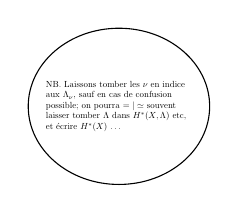
\begin{tikzpicture}[scale=.32,transform shape]
\draw (0,0) ellipse (3.6cm and 3.1cm);
\node[text width=5.8cm,align=left] at (0,0) {\uline{NB.} Laissons tomber les $\nu$ en indice aux $\Lambda_\nu$, sauf en cas de confusion possible; on pourra $\unsure{=|\simeq}$ souvent laisser tomber $\Lambda$ dans $H^*(X,\Lambda)$ etc, et écrire $H^*(X)$ \ldots};
\end{tikzpicture}}}

\scanpage{131}
\mspage{V.2}
% archive sheet number: 130

% L01-02 left upper margin, pencilled and slanted
% margin note written slanted
\margin{\figure{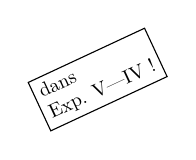
\begin{tikzpicture}[scale=.7,transform shape]
\node[draw,rotate=25,align=left] {dans\\ Exp. \unsure{V|IV} !};
\end{tikzpicture}}}

% L01-06
\deleted{\unsure{1.4}}1.1. Nous allons donner une interprétation frappante des fibres $(\underline{\Psi}_{\unsure{\alpha|\nu}}^{(q)})_{\overline{x}}$ des faisceaux introduits dans (\inserted{\uline{III}} 2.6), où $\overline{x}$ est un point géométrique de $\widetilde{X}_0$. Pour ceci, introduisons le localisé strict $\overset{\deleted{\unsure{\sim}}}{X}'$ de $\widetilde{X}$ en $\overline{x}$; \deleted{\unsure{et}}\inserted{nous pouvons \unsure{identifier}} le localisé strict correspondant de $S$ égal à $\widetilde{S}$, du fait qu'on a un morphisme canonique

% L05 margin enclosed in a box
\margin{\figure{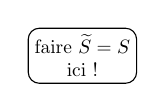
\begin{tikzpicture}[scale=.7,transform shape]
\node[draw,rounded corners,align=center] {faire $\widetilde{S}=S$\\ ici !};
\end{tikzpicture}}}

% L07
\[
\overset{\deleted{\sim}}{f}' : \overset{\deleted{\sim}}{X}'\longrightarrow\widetilde{S}
\tag*{\deleted{\unsure{(0.1.1)}} (1.1.1)}
\]

% L08-10
Si $\overset{\deleted{\sim}}{U}'$ est l'image inverse de $U$ dans $\overset{\deleted{\sim}}{X}'$, c'est un ouvert de la fibre générique $\overset{\deleted{\sim}}{X}'_{\widetilde{\eta}}$ de $\overset{\deleted{\sim}}{f}'$ sur $\widetilde{S}$ :
\[
\overset{\deleted{\sim}}{U}'\subset\overset{\deleted{\sim}}{X}'_{\widetilde{\eta}}.
\tag*{\unsure{(1.1.2)}}
\]

% L11-12
Ceci posé, le \deleted{\unsure{calcul du}} calcul habituel des fibres de faisceaux \inserted{$R^{\unsure{q|i}}g_*$} (SGA 4 \uline{VIII}\quad) montre qu'on a

% L13 bottom left margin, slanted and enclosed
% margin note written slanted
\margin{\figure{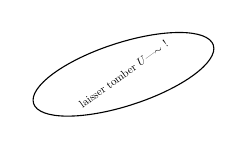
\begin{tikzpicture}[scale=.4,transform shape,rotate=18]
\draw (0,0) ellipse (3cm and 1cm);
\node[rotate=18] at (0,0) {laisser tomber \unsure{$U$|$\sim$} !};
\end{tikzpicture}}}

\scanpage{132}
\mspage{V.3}
% archive sheet number: 131

% L01-04 diagram at top
\diagram{\begin{tikzcd}[ampersand replacement=\&,column sep=small,row sep=large]
\& \& \overset{\deleted{\unsure{\sim}}}{X}'\arrow[dl] \& \overset{\deleted{\sim}}{X}'_{\widetilde\eta}\arrow[l,hook]\arrow[dl] \& \overset{\deleted{\sim}}{U}'\arrow[l,hook]\arrow[dl] \& \overline U'\arrow[l]\arrow[dl] \\
X\arrow[d] \& \widetilde X\arrow[l]\arrow[d] \& \widetilde X_{\widetilde\eta}\arrow[l,hook]\arrow[d] \& \widetilde U\arrow[l,hook]\arrow[d,dashed,no head] \& \overline U\arrow[l]\arrow[d]\arrow[lll,bend left=17,"g"'] \& \\
S \& \widetilde S\arrow[l] \& \widetilde\eta\arrow[l,no head] \& \deleted{\unsure{\overline\eta|\widetilde\eta}}\widetilde\eta\arrow[l] \& \overline\eta\arrow[l] \&
\end{tikzcd}}

% L05-07
un isomorphisme canonique
\[
(\underline\Psi_\nu^{(q)})_{\overline x}\simeq\deleted{H^q(\unsure{\overline U'\times_{\widetilde X}\overline U},\unsure{\Lambda})}\inserted{H^q(\overline U',\Lambda_\nu)},\quad\text{où}\quad\overline U'\simeq X'\times_{\widetilde X}\overline U.
\]

% L08-10
Et comme on a
\[
X'\times_{\widetilde X}\overline U\simeq U'\times_{\widetilde U}\overline U\simeq U'\times_{\widetilde\eta}\overline\eta,\quad-
\]
on trouve finalement
\[
\deleted{\unsure{H^q}}(\underline\Psi_\nu^{(q)})_{\overline x}\simeq H^q(\overline U',\Lambda_\nu),\quad\overline U'=U'\otimes_{\widetilde\eta}\overline\eta=U'\otimes_{\widetilde K}\overline K.
\tag*{\unsure{(1.1.3)}}
\]

% L11-14
Si par exemple $U=X_\eta$ (cas de loin le plus important), on trouve
\[
(\underline\Psi_\nu^{(q)})_{\overline x}\simeq H^q(X'\times_{\widetilde S}\overline\eta,\Lambda_\nu),
\tag*{(1.2)}
\]

% L15-19
i.e. \uline{\unsure{les fibres|la fibre} du faisceau} $\deleted{\unsure{(}}\underline\Psi_\nu^{(q)}\deleted{\unsure{)_{\overline x}}}$ en le point \uline{géom.} $\overline x$ \uline{de} $\widetilde X$ \deleted{sont} \uline{n'est autre que le} \uline{$q$.ième groupe de cohomologie} \inserted{(à coeff. dans $\Lambda_\nu$)} \uline{de la fibre} \inserted{\uline{géométrique}} \uline{générique sur} $\widetilde S$ \uline{du localisé strict} $X'$ \uline{de} $X$ en $\overline x$.

% L20-24 left margin, written slanted along edge
% margin note written slanted
\margin{(De façon imagée, on peut dire que les relations globales entre les deux fibres géométriques $X_{\overline s}$, $X_{\overline\eta}$ se \deleted{\unsure{reflètent|réflètent}}\inserted{\unsure{réfèrent|réduisent}} par les développements précédents aux propriétés des fibres géométriques locales \inserted{\unsure{(i.e. des fibres} génériques du morphisme $X'\longrightarrow\widetilde S$ entre localisés stricts de $X$ et $S$).};)}

% L20 cancelled line above final paragraph
\deleted{\unsure{La même méthode donne} \unsure{pour} les relations,}

% L21-23
Compte tenu des \deleted{\unsure{mêmes}} relations (2.8), on \deleted{\unsure{2}} en conclut des expressions correspondantes pour les

% L24 bottom-edge addition transcribed at the end of the slanted note above;
% the curved leader joins its lower end. Attachment is recorded in the doubts file.

\mspage{V.4}
% archive sheet number: 131A

% L25-26 continuation on second physical sheet
fibres $(\underline\Phi_\nu^{(q)})_{\overline x}$ des faisceaux de cycles évanescents.

% L27-28
\deleted{\unsure{2} Lorsque} Le même argument donne les relations
\[
(\underline\Psi_\nu^{(q)}\deleted{\unsure{)}}_{\mathrm{tame}})_{\overline x}\simeq H^q(U'\otimes_{\widetilde K}\overline K_t),
\tag*{\deleted{\unsure{(2.10)}}}
\]

% L29-31
en particulier si $U=X_\eta$, ceci \deleted{devient} prend la forme
\[
(\underline\Psi_{\nu\,\mathrm{tame}}^q)_{\overline x}=H^q(X\otimes_{\widetilde S}\operatorname{Spec}\overline K_t)
\tag*{\unsure{(1.3)|(1.B)}}
\]
\unsure{;|?} :

% L32 second sheet bottom cancellation
\deleted{\unsure{on a}}

